%!Tex Root = ../Tutorat1.tex
% ./Packete.tex
% ./Design.tex
% ./Deklarationen.tex
% ./Aufgabe1.tex
% ./Aufgabe2.tex
% ./Bonus.tex

\section{Task 3 - Interrupt and Polling}

\setcounter{task}{1}

\begin{frame}[fragile]{Task 3 - Interrupts and Polling}{Task 3}
  \begin{solution}
    \begin{columns}
      \begin{column}{0.8\textwidth}
        \begin{itemize}
          \item Computation time C for the event: $\frac{100}{48 \cdot 10^6 Hz} = 2.0833\mu s$
          \item The maximum response time in the worst case is $P + C$. This time should not exceed our deadline of $10 \mu s$
          \item Therefore, we have $P + 2.0833\mu s \leq 10\mu s \Longleftrightarrow P \leq 7.9167\mu s$
          \item Since our polling period may not be shorter than the computation time we obtain $P \geq 2.0833\mu s$. Therefore, our range is $P \in [2.0833\mu s, 7.9167\mu s]$
        \end{itemize}
      \end{column}
    \end{columns}
  \end{solution}
\end{frame}

\begin{frame}{Solution a:}{Task 3}
  \centering
  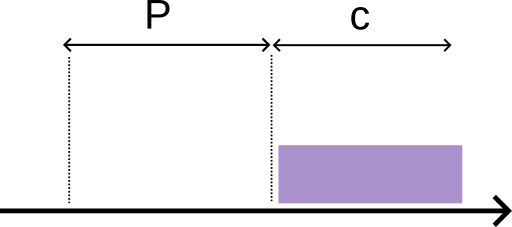
\includegraphics[height=0.4\paperheight]{figures/task3-a.png}
\end{frame}

\if\preview0{
\begin{frame}[fragile]{Task 3 - Interrupts and Polling}{Task 3}
  \begin{solution}
    \begin{columns}
      \begin{column}{0.8\textwidth}
        \begin{itemize}
          \item In this setting, the worst case occurs if an interrupt delays our event computation.
          \item Our maximum response time is $P + C + H$ where $H$ is the overhead time required to process the interrupt.
          \item Because our event takes 100 cycles, and the time between two interrupts is 140 cycles, there can be at most one interrupt within the processing of our event.
          \item Thus, we require 40 more cycles in the worst case, taking $\frac{40}{48 \cdot 10^6Hz} = 0.8333\mu s$
          \item Calculating the range like in (a), we obtain $P \in [2.9167\mu s, 7.0833\mu s]$
        \end{itemize}
      \end{column}
    \end{columns}
  \end{solution}
\end{frame}

\begin{frame}{Solution b:}{Task 3}
  \centering
  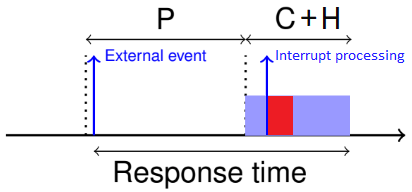
\includegraphics[height=0.4\paperheight]{figures/task3-b.png}
\end{frame}

\begin{frame}[fragile]{Task 3 - Interrupts and Polling}{Task 3}
  \begin{solution}
    \begin{columns}
      \begin{column}{0.8\textwidth}
        \begin{itemize}
          \item Let E be the total cycles of computation within one polling period. Let k be the amount of interrupts that occured during the processing of our event.
          \item We have that $E = 100 + 40 \cdot k$
          \item 1. To meet the deadline, we require $\frac{E}{48 \cdot 10^6Hz} + P \leq 10\mu s$
          \item 2. To finish the polling task before a new period $P \geq \frac{E}{48 \cdot 10^6Hz}$
          \item Through this we can derive that $2 \cdot \frac{E}{48 \cdot 10^6Hz} \leq 10\mu s \Rightarrow E \leq 240 Cycles$
        \end{itemize}
      \end{column}
    \end{columns}
  \end{solution}
\end{frame}

\begin{frame}[fragile]{Task 3 - Interrupts and Polling}{Task 3}
  \begin{solutionnoinc}
    \begin{columns}
      \begin{column}{0.8\textwidth}
        \begin{itemize}
          \item Assuming the largest feasible value of E, we have $k = \frac{240 - 100}{40} = 3.5$
          \item This means at most 3 interrupts can be processed fully during the processing of one event. In total this takes $\frac{100 + 40 \cdot 3}{40} = 4.583\mu s$ time.
          \item The minimum feasible time between two interrupts is $T = 4.583\mu s/3 = 1.528\mu s$
          \item The feasible range for the polling period is $P \in [4.583\mu s, 5.147\mu s]$
        \end{itemize}
      \end{column}
    \end{columns}
  \end{solutionnoinc}
\end{frame}
\fi
